%\documentclass[final]{article}
\documentclass[]{article}
\usepackage{geometry}
\geometry{
	a4paper,
	total={170mm,257mm},
	left=0.75in,
	top=0.75in,
	right=0.75in,
	bottom=1in,
}
\newcommand{\extramargin}[1]{}
%\newcommand{\extramargin}[1]{
%	\setlength{\paperwidth}{250mm}
%	\setlength{\evensidemargin}{-15mm}
%	\setlength{\oddsidemargin}{-15mm}
%}
\usepackage{gensymb}
\usepackage{lipsum}
\usepackage{graphicx}
\usepackage{epstopdf, epsfig}
\usepackage{amsmath}
\usepackage[url=false,
backend=bibtex,
style=authoryear-comp,
giveninits=true,
doi=true,
isbn=true,
backref=false,
dashed=false,
maxcitenames=2,
maxbibnames=99,
natbib=true]{biblatex}
\DeclareNameAlias{author}{last-first}
\DeclareFieldFormat
[article,inbook,incollection,inproceedings,patent,thesis,
unpublished,techreport,misc,book]
{title}{#1}
\renewcommand*{\revsdnamepunct}{}
\renewbibmacro{in:}{}
\usepackage{xpatch}
\xpatchbibmacro{date+extradate}{%
	\printtext[parens]%
}{%
	\setunit*{\space}%
	\printtext%
}{}{} 


\addbibresource{../Main/ViscousDropImpact_v2.bib}
\nonfrenchspacing
\setlength\parindent{0pt}
\usepackage{siunitx}
\usepackage{xcolor}
\usepackage{mathrsfs}
\usepackage[colorlinks,citecolor=purple]{hyperref}
\newcommand*\blue{\textcolor{blue}}
\newcommand*\red{\textcolor{red}}
\newcommand{\VS}[1]{{\textcolor{orange}{#1}}}

\renewcommand{\thefigure}{R\arabic{figure}}

\usepackage[obeyFinal,colorinlistoftodos, textwidth=60mm, shadow]{todonotes}
% todonotes specific macros begin!
\newcommand{\todoInsertref}[2]{\todo[color=green!40, #1]{#2}}
\newcommand{\todoExplaininDetails}[2]{\todo[color=orange!40, #1]{#2}}
\newcommand{\todoUrgent}[2]{\todo[color=red!40, #1]{#2}}
\newcommand{\todoSansUrgent}[2]{\todo[color=yellow!40, #1]{#2}}
\extramargin
%% todonotes specific macros end!

%opening
\title{Reply to Referee 1}
\author{Vatsal Sanjay, Bin Zhang, Cunjing Lv, and Detlef Lohse}
\date{}
\begin{document}
	\maketitle
	
\textit{The authors describe a combined numerical and experimental study on the influence of Weber and Ohnesorge number on the peak forces (and their associated timing) associated with droplet impact and rebound on a non-wetting, rigid, planar surface. Scaling arguments are proposed throughout to help rationalize the trends observed in the data. This work represents a direct extension of work previously published by the same group (Zhang et al. PRL 2022) wherein they identified the possibility of two peaks in the impact force evolution associated with the initial impact and retraction stages. Overall, the manuscript is well written and easy to follow. However I do have some major and minor concerns that are described in what follows.}\\[2mm]

We thank the referee for carefully reading our manuscript and providing valuable feedback and suggestions. We have reviewed the referee's comments and made changes based on their suggestions. Below, we offer a point-to-point reply to each of the referee's comments and include the changes made in the manuscript. The referee's comments are in italics, and our replies are in plain black. Changes in the manuscript are highlighted in orange.

\begin{enumerate}
	\item \textit{Apart from Figure 2 (which appears to be the previously published data from Figure 1 in Zhang et al. (PRL 2022)), there is very little direct comparison between experiment and simulation. Now that the parameter space has been significantly extended from prior work, I would have expected similar direct force versus time comparisons and droplet shape profiles spanning the new range of parameters to validate the simulation. Comparisons similar to that in Figure 2 should be included throughout when the various parameter various regimes are introduced and discussed.}\\[0.5mm]
	
	Yes, it is correct that the earlier version of figure 2 summarized the results previously published in \citet{zhang2022impact}. To extend the comparison at different Ohnesorge numbers $Oh$, we have added two additional $F(t)$ curves in figure 2 (see figure~\ref{fig:summary}). Furthermore, throughout the manuscript, we present experimental data wherever available (see figures 3 and 7). 

	\begin{figure}
		\centering
		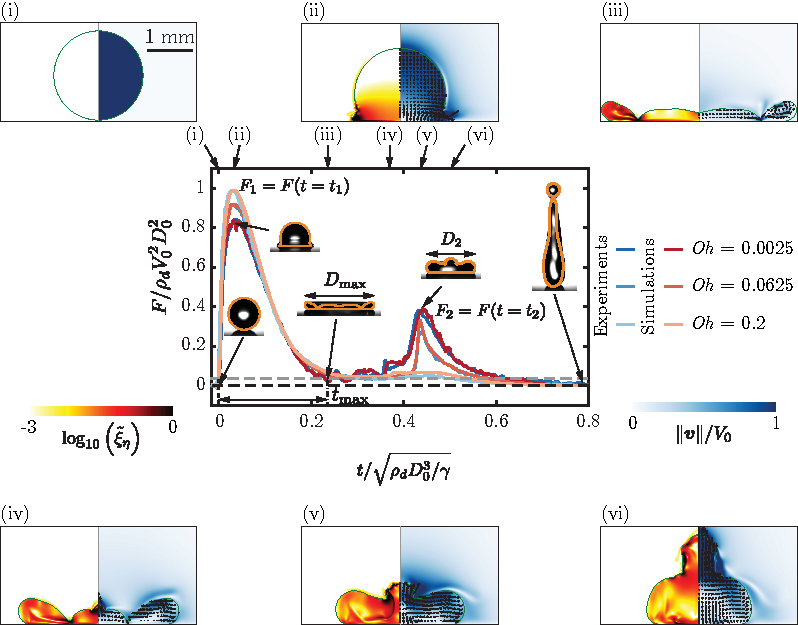
\includegraphics[width=\textwidth]{../Main/Figures/Figure1_summary_v5.pdf}
		\caption{\VS{Comparison of the drop impact force $F(t)$ obtained from experiments and simulations for the three typical cases with impact velocity $V_0 = 1.2\,\si{\meter}/\si{\second}, 0.97\,\si{\meter}/\si{\second}, 0.96\,\si{\meter}/\si{\second}$, diameter $D_0 = 2.05\,\si{\milli\meter}, 2.52\,\si{\milli\meter}, 2.54\,\si{\milli\meter}$, surface tension $\gamma = 72\,\si{\milli\newton}/\si{\meter}, 61\,\si{\milli\newton}/\si{\meter}, 61\,\si{\milli\newton}/\si{\meter}$ and viscosity $\eta_d = 1\,\si{\milli\pascal\second}, 25.3\,\si{\milli\pascal\second}, 80.2\,\si{\milli\pascal\second}$. These parameter give $Oh = 0.0025, 0.0625, 0.2$ and $We = 40$.
			For the three cases, the two peak amplitudes, $F_1/\rho_dV_0^2D_0^2 \approx$ 0.82, 0.92, 0.99 at $t_1 \approx 0.03\sqrt{\rho_dD_0^3/\gamma}$ and $F_2/\rho_dV_0^2D_0^2 \approx$ 0.37, 0.337, 0.1 at $t_2 \approx 0.42\sqrt{\rho_dD_0^3/\gamma}$, characterize the inertial shock from impact and the Worthington jet before takeoff, respectively. 
			The drop reaches the maximum spreading at $t_{\text{max}}$ when it momentarily stops and retracts until $t_3 \approx 0.8\sqrt{\rho_dD_0^3/\gamma}$ when the drop takes off ($F = 0$).
			Six instances are further elaborated through numerical simulations for ($We = 40, Oh = 0.0025$), namely (i) $t = 0\,\si{\milli\second}$ (touch-down), (ii) $t = 0.37\,\si{\milli\second}$ ($t_1$), (iii) $t = 2.5\,\si{\milli\second}$ ($t_{\text{max}}$), (iv) $t = 3.93\,\si{\milli\second}$ ($\approx 0.85t_2$), (v) $t = 4.63\,\si{\milli\second}$ ($t_2$), and (vi) $t = 5.25\,\si{\milli\second}$ ($\approx 1.15t_2$). 
			We stress the excellent agreement between experiments and simulations without any free parameters. The insets show representative snapshots at specific time instants overlaid with the drop boundaries from simulations in orange, also revealing good agreement. 
			The left part of each numerical snapshot shows the dimensionless local viscous dissipation function $\tilde{\xi}_\eta \equiv \xi_\eta D_0/\left(\rho_dV_0^3\right) = 2Oh\left(\boldsymbol{\tilde{\mathcal{D}}:\tilde{\mathcal{D}}}\right)$, where, $\boldsymbol{\mathcal{D}}$ is the symmetric part of the velocity gradient tensor, on a $\log_{10}$ scale and the right part the velocity field magnitude normalized with the impact velocity. The black velocity vectors are plotted in the center of mass reference frame of the drop to clearly elucidate the internal flow.}}
		\label{fig:summary}
	\end{figure}
	
	For the high Ohnesorge number regime ($Oh \gg 1$) discussed in Figure 5, we, unfortunately, do not have corresponding experimental data as we used water-glycerol mixtures in the experiments, which can at most be 1000 times (100\% by weight of glycerine) more viscous than water. However, to provide an additional comparison, we have added a new panel (Figure 5c, see figure~\ref{fig:F1Anatomy_2}) comparing our results with those from \citet{Gordillo2018, cheng2021drop}. This comparison focuses on the relationship between the first peak force $F_1$ and the impact Reynolds number $Re = \rho_dV_0D_0/\eta_d$.
	
	\begin{figure}
		\centering
		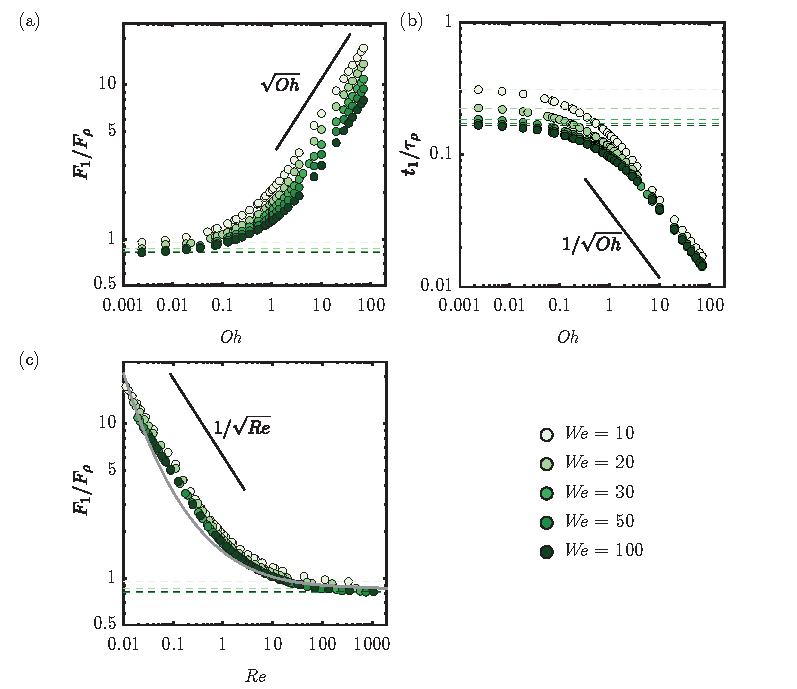
\includegraphics[width=\textwidth]{../main/Figures/ForceTimeVersusOhnesorge.pdf}
		\caption{\blue{Anatomy of the first impact force peak amplitude for viscous impacts from our numerical simulations: the $Oh$ dependence of  (a) the magnitude $F_1$ normalized by the inertial force scale $\rho_dV_0^2D_0^2$ and (b) the time $t_1$ to reach the first force peak amplitude normalized by inertial timescale $\tau_\rho = D_0/V_0$}. \VS{(c) The $Re$ dependence of the magnitude $F_1$ normalized by the inertial force scale $\rho_dV_0^2D_0^2$ as compared to the (implicit) theoretical calculation of \citet{Gordillo2018}.} \blue{The black line corresponds to the scaling relationship described in \S~3.2. The Weber number is color-coded.}}
		\label{fig:F1Anatomy_2}
	\end{figure}
	
	
	\item \textit{Error bars (both horizontal and vertical) for the experiments should be included throughout whenever experimental data is presented. If smaller than the data points, this should be noted. Furthermore, a discussion of any error analysis is completely lacking. For the error bars that are included, do these account for multiple trials? Parameter uncertainties? Measurement uncertainties? Such a discussion, with errors quantified (and methods used to assess the errors), must be included. In particular, the resolution of the force sensor (reported as 0.5 mN) should be indicated when force measurements are presented, including in Figure 2.}\\[0.5mm]
	
	Thank you for highlighting the importance of error analysis and the need for a more comprehensive discussion of error quantification in our manuscript. We appreciate your suggestions. Indeed, we have included the error bars wherever experimental data are reported. For the cases where the error bars are not visible, the error bar is smaller than the data points. For more details regarding the error quantification, we refer the readers to the supplementary material of \citet{zhang2022impact}. We have added this clarification in the experimental method section:
	
	\S~\red{2.1:}\\
	\VS{Throughout the manuscript, the error bars account for repeated trials and are visible if they are larger than the marker size. We refer the readers to the supplementary material of \citet{zhang2022impact} for further details of the experimental setup.}\\[0.5mm]
	
	We have also added a dashed gray horizontal line in figure 2 to mark the resolution of the force sensor. 
	
	\item \textit{Furthermore, the dimensional parameters of the experiments performed need to somehow be specified or indicated. The authors mention a range of droplet sizes, viscosities, and impact speeds, and so We and Oh do not uniquely defined the experimental realizations reported. This specificity is critical for repeatability and future comparisons that might be made.}\\[0.5mm]
	
	Thank you for raising this important point about the need to specify the dimensional parameters of the experiments. We appreciate the emphasis on the importance of this information for repeatability and future comparisons. We vary the impact velocity by changing the release height of the drops above the substrate and change the viscosity by using different water-glycerol mixtures. Such a protocol allows us to vary the viscosity by almost two orders of magnitude, yet maintaining a fairly constant density and surface tension. Consequently, the Weber number $We$ can be interpreted as a dimensionless impact velocity and the Ohnesorge number $Oh$ as a dimensionless viscosity. We have modified the text to clarify the experimental protocol and provide more details on the dimensional parameters:
	
	\S~\red{2.1:}\\
	\VS{The properties of the impacting drop are controlled using water-glycerol mixtures with viscosities $\eta_d$ varying by almost two orders of magnitude, from $1\,\si{\milli\pascal}\si{\second}$ to $80.2\,\si{\milli\pascal}\si{\second}$, yet maintaining a fairly constant surface tension $\gamma$ and density $\rho_d$ around $61\,\si{\milli\newton}/\si{\meter}$ and $1000\,\si{\kilo\gram}/\si{\cubic\meter}$, respectively \citep{cheng2008formula, volk2018density, Jha2020}. Using other liquids like silicone oil could allow for a wider viscosity variation if used with a superamphiphobic substrate \citep{deng2012candle}. The drop diameter $D_0$ is controlled between $2.05\,\si{\milli\meter}$ and $2.76\,\si{\milli\meter}$ by pushing it through a calibrated needle. Throughout this work, we use drops with diameter $2.54 \pm 0.02\,\si{\milli\meter}$ unless otherwise stated. Consequently, changing the viscosity of the drop determines the Ohnesorge number ($Oh$, see~1.2). The Weber number ($We$, see~1.1) is set using the impact velocity $V_0$ varying between $0.38\,\si{\meter}/\si{\second}$ and $2.96\,\si{\meter}/\si{\second}$ by changing the release height of the drops above the substrate. Lastly, we keep the Bond number ($Bo$, see~1.3) fixed at 1 throughout the manuscript. In our system, the relevance of gravity is characterized by the dimensionless Froude number $Fr = V_0^2/gD_0 = We/Bo$ comparing inertia with gravity. Throughout this manuscript, $Fr > 1$ and gravity's role is sub-dominant compared to inertia.}
	
	This expanded description provides several key pieces of information:
	\begin{enumerate}
		\item The range of viscosities ($1,\si{\milli\pascal}\si{\second}$ to $80.2,\si{\milli\pascal}\si{\second}$) achieved using water-glycerol mixtures.
		\item The relatively constant surface tension ($61,\si{\milli\newton}/\si{\meter}$) and density ($1000,\si{\kilo\gram}/\si{\cubic\meter}$) of these mixtures.
		\item The range of drop diameters ($2.05,\si{\milli\meter}$ to $2.76,\si{\milli\meter}$) and the typical diameter used ($2.54 \pm 0.02,\si{\milli\meter}$).
		\item The range of impact velocities ($0.38,\si{\meter}/\si{\second}$ to $2.96,\si{\meter}/\si{\second}$) achieved by varying the release height.
	\end{enumerate}

	We also clarify that the Ohnesorge number ($Oh$) is uniquely determined by the drop viscosity, while the Weber number ($We$) is set by the impact velocity.

	By providing these details, we aim to ensure that our experiments can be readily reproduced and that future comparisons can be made with a clear understanding of the dimensional parameters involved. We believe this additional information significantly enhances the repeatability and usefulness of our work.
	
	We have also modified the caption of figure 2 (see figure~\ref{fig:summary}) to clarify the drop impact parameters. 
		
	\item \textit{Is gravity included in the simulations? If so, the Bond number in simulations should be specified, as We and Oh alone do not uniquely define the non-dimensional problem. The authors show that droplet rebound can be affected by finite Bond number effects in their very recent prior work (Sanjay et al. JFM 2023), so at least some discussion on the role of gravity should be included.}\\[0.5mm]
	
	Thank you for raising this important question about the role of gravity in our simulations and the need to specify the Bond number. In deed, in \citet{sanjay_chantelot_lohse_2023}, we highlight the potential influence of finite Bond number on the bouncing--no-bouncing transition on a non-wetting surface. 
	
	To address your concerns, we have made the following revisions to the manuscript:
	
	\begin{enumerate}
		\item We have clarified that gravity is indeed included in our simulations and that the Bond number (based on the drop's diameter) $Bo = \rho_dgD_0^2/\gamma$ is fixed at 1 throughout the study. This information has been added to the manuscript as follows:
		
		\S~\red{2.1:}\\
		\VS{Throughout the manuscript, we keep the Bond number ($Bo$, see~(1.3)) fixed at 1 in our simulations, which include the effects of gravity.}
		
		\item We have updated Figure 10 to indicate that the critical $Oh$ to suppress bouncing is 0.53 for the chosen $Bo$ of 1. Note that in \citet{sanjay_chantelot_lohse_2023}, we use the radius $R_0 = D_0/2$ as the length scale to get $Oh_c + Bo_c \approx 1$. 
		
		\item We have introduced the dimensionless Froude number $Fr = V_0^2/gD_0 = We/Bo$, which compares inertia with gravity. We clarify that throughout the manuscript, $Fr > 1$, indicating that the role of gravity is sub-dominant compared to inertia. This discussion has been added as follows:
		
		\S~\red{2.1:}\\
		\VS{In our system, the relevance of gravity is characterized by the dimensionless Froude number $Fr = V_0^2/gD_0 = We/Bo$, which compares inertia with gravity. Throughout this manuscript, $Fr > 1$, indicating that the role of gravity is sub-dominant compared to inertia.}
	\end{enumerate}
	
	\item \textit{The title needs to be rewritten. The authors demonstrate that capillarity also plays a crucial role, and seem to ignore gravity throughout the present work anyways (i.e. gravity doesn’t dictate impact forces here, because it is assumed). Furthermore, the title does not specify the nature of the substrate, which is a specific case. I would suggest something along the lines of ``Impact forces of droplets on non-wetting planar surfaces" or similar.}
	
	We agree with the reviewer that the title was misleading. Of course, all three: inertia, capillarity, and viscosity, play a role. Indeed, we have studied the role of inertial and capillarity in \citet{zhang2022impact}. We have now changed the title of the paper to:
	
	\VS{The role of viscosity on drop impact forces}
	
	\item \textit{What are the receding and advancing contact angles for the experimental surfaces used? The experimental substrate is not truly non-wetting (in contrast to the simulation), so this should be clearly described.}\\[0.5mm]
	
	Yes, the reviewer is correct. The substrate is not truly non-wetting in the experiments. We have added this in the revised manuscript along with the advancing and the receding contact angles. 
	
	\S~\red{2.1:}\\
	 \VS{For water drops, such a surface is coated with silanized silica nanobeads with a diameter of $20\,\si{\nano\meter}$ (Glaco Mirror Coat Zero; Soft99) resulting in the advancing and receding contact angles of $167 \pm 2^{\circ}$ and $154 \pm 2^{\circ}$, respectively \citep{Gauthier2015, Li2017}. On the other hand, for viscous aqueous glycerin drops, the upper surface is coated with an acetone solution of hydrophobic beads (Ultra ever Dry, Ultratech International, a typical bead size of 20 nm), resulting in the advancing and receding contact angles of $166 \pm 4^{\circ}$ and $159 \pm 2^{\circ}$, respectively \citep{Jha2020}.}
	
	\item \textit{In the experiments, are the droplets arriving at the surface without residual oscillation? Particular for the small We, small Oh cases, I would expect this is not the case. This should be discussed.}
	
	Thank you for raising this important point about the potential influence of residual oscillations in the drop as they arrive at the surface, particularly for cases with small Weber and Ohnesorge numbers. We agree that this aspect of the experimental setup deserves discussion in the manuscript.
	To address this concern, we have added the following text to the manuscript:
	
	\S~\red{2.2:}\\
	\VS{At $t = 0$, in our simulations, we release a spherical drop whose south pole is $0.05D_0$ away from the substrate and is falling with a velocity $V_0$. It is important to note that the drop may not be perfectly spherical and may have residual oscillations as they are released from the needle and arrive at the substrate. These oscillations are expected to be more pronounced for cases with small Weber and Ohnesorge numbers. The exact shape of the drop just before impact can influence the impact dynamics \citep{thoraval-2013-jfm, yun2017bouncing}. However, we suspect that the influence of these shape variations is captured, at least in part, by the error bars in the experimental data, which are derived from repeated trials under the same nominal conditions.}
	
	By acknowledging the possibility of residual oscillations and their potential influence on the impact dynamics, we aim to provide a more complete and transparent description of the experimental setup. We also highlight that the error bars in the experimental data, which are derived from repeated trials, likely account for some of the variability introduced by these shape variations.
	
	The inclusion of this discussion helps readers to better understand the limitations and uncertainties inherent in the experimental setup, and it provides important context for interpreting the results. We have also added references to relevant literature \citep{thoraval-2013-jfm, yun2017bouncing} that further explore the influence of drop shape on impact dynamics.
	
	\item \textit{How are the density, viscosity, and surface tension of the various water-glycerol mixtures determined? These also need to be reported.}
	
	We use the protocol described in \citet{cheng2008formula, volk2018density}. We have added a new table~\ref{tab:table00} with all the material properties (density, viscosity, and surface tension) of the water-glycerol mixtures used in this work. 
	
	\begin{table}
		\begin{center}
			\def~{\hphantom{0}}
			\begin{tabular}{lccc}
				glycerol & $\rho_d$ & $\eta_d$  & $\gamma$\\
				(wt \%) &(kg/m$^{3}$) &(mPa.s)& (mN/m)\\[3pt]
				0 & 1000 & 1 & 72 \\
				50 & 1124 & 5 & 61 \\
				63 & 1158 & 10 & 61 \\
				74 & 1188 & 25.3 & 61 \\
				80 & 1200 & 45.4 & 61 \\
				85 & 1220 & 80.2 & 61 \\
			\end{tabular}
			\caption{\VS{Properties of the water-glycerol mixtures used in the experiments. $\rho_d$ and $\eta_d$ are the density and viscosity of the drop, respectively and $\gamma$ denotes the liquid-air surface tension coefficient. These properties are calculated using the protocol provided in \citet{cheng2008formula, volk2018density}.}}
			\label{tab:table00}
		\end{center}
	\end{table}

	\item \textit{Some details on the numerical implementation are left out. In particular, the computational domain size and initial conditions should be specified.}
	
	We have added these details in the revised manuscript: 
	
	\S~\red{2.2:}\\
	\VS{The domain boundaries are far enough from the drop not to influence its impact process ($\mathcal{L}_\text{max} \gg D_0$, $\mathcal{L}_\text{max} = 8R$ in the worst case). At $t = 0$, in our simulations, we release a spherical drop whose south pole is $0.05D_0$ away from the substrate and is falling with a velocity $V_0$. It is important to note that the drops may not be perfectly spherical and may have residual oscillations as they are released from the needle and arrive at the substrate. These oscillations are expected to be more pronounced for cases with small Weber and Ohnesorge numbers. The exact shape of the drop just before impact can influence the impact dynamics \citep{thoraval-2013-jfm, yun2017bouncing}. However, we suspect that the influence of these shape variations is captured, at least in part, by the error bars in the experimental data, which are derived from repeated trials under the same nominal conditions.}
	
	\item \textit{The authors ignore the role of the air film in the dynamics on the grounds that the air-based Ohnesorge number is small, however the air gap can become extremely small and thus it is not clear that the drop diameter is the relevant length scale in assessing the viscous forces in the air. Furthermore, this is contrast to prior work on non-wetting impacts (such as Kolinski et al. (EPL 2014)) that argues viscous effects in the thin gas layer can play a role in the liquid dynamics. This should be discussed.}
	
	Thank you for raising this important point about the role of the air film in the drop impact dynamics. We appreciate the opportunity to discuss this aspect further and clarify its relevance to our work.
	
	We acknowledge that our treatment of the air film, based on the small air-based Ohnesorge number, may only partially capture the complexity of the viscous forces in the thin gas layer. The reviewer rightly points out that the drop diameter is not the most appropriate length scale for assessing these forces, especially when the air gap is extremely thin. This approach contrasts with some prior work on non-wetting impacts, such as \citet{kolinski-2014-epl}, which argues for the significance of viscous effects in the thin gas layer on the liquid dynamics. In fact, the air layer has two important contributions: 
	
	\begin{enumerate}
		\item It prevents the contact between the falling drop and the solid surface. 
		\item It might lead to dissipation owing to the large velocity gradients. 
	\end{enumerate}
	
	To understand the relative importance of these two effects, we have recently conducted direct numerical simulations and compared the results with experiments on various surfaces, including superhydrophobic surfaces \citep{sanjay_chantelot_lohse_2023}, atomically smooth viscous films \citep{sanjay2023drop}, and even other drops \citep{ramirez2020lifting}. Our findings suggest that, for the macroscopic observables, the primary contribution of the air film is to prevent contact between the drop and the substrate. In contrast, the dissipation inside the air film itself does not play a significant role in the parameter range we study. This feature is particularly notable for large Weber numbers ($We$) where substrate-independent bouncing ceases.
	Despite the high-velocity gradients in the air film, we propose that the dissipation inside the drop dominates in all the cases we have examined. The small volume and low air viscosity limit the dissipation it can create, in contrast to the findings of previous works like \citet{kolinski-2014-epl}. However, we also acknowledge the complexity of modeling the air film, especially considering the extremely small Knudsen numbers involved. In such cases, a hybrid method \citep{chubynsky-2020-prl, sprittles2024gas} might provide a more accurate description.
	
	We have added a discussion of these points in the revised manuscript to provide a more comprehensive discussion of the role of the air film in drop impact dynamics and to address the apparent contrast with prior work. We thank the reviewer for highlighting this important aspect and helping us improve the clarity and completeness of our manuscript.
	
	\S~\red{2.2:}\\
	\VS{To ensure a perfectly non-wetting surface, we impose a thin air layer (minimum thickness $\sim \Delta/2$) between the drop and the substrate. This air layer prevents direct contact between the liquid and solid \citep{kolinski-2014-epl, sprittles2024gas}, effectively mimicking a perfectly non-wetting surface. The presence of this air layer is crucial for capturing the dynamics of drop impact on superhydrophobic surfaces, as it allows for the formation of an air cushion that can significantly affect the spreading and rebound behavior of the drop \citep{ramirez2020lifting, sanjay_chantelot_lohse_2023}.
	While this approach does not fully resolve the microscopic dynamics within the air layer itself, such as the high-velocity gradients and viscous dissipation inside the gas film once it thins below a critical size ($\sim 10\Delta$), it has been shown to accurately capture the macroscopic behavior of drop impact in the parameter range of interest \citep{ramirez2020lifting, sanjay2023drop, alventosa2023inertio, garcia2024skating}. We refer the readers to \citet{VatsalThesis} for discussions about this \lq\lq precursor\rq\rq, air film method and to \citet{popinet-basilisk, vatsal_sanjay_2023_7598181, zhang2022impact} for details on the numerical framework.}
	
	
	\item \textit{Figure 5 does not include any experimental data. This should be explained. Perhaps the high Oh regime is not accessible with the droplet sizes and fluids used?}
	
	Thank you for raising this important point about the experimental data in Figure 5. We appreciate your suggestion to consider using other liquids, such as silicone oil, to probe a wider range of viscosity and Ohnesorge number ($Oh$).
	In our experiments, we focused on using water-glycerol mixtures, which allowed us to explore two orders of magnitude in $Oh$. While silicone oil could indeed provide access to a broader viscosity range, it would require the use of superamphiphobic surfaces \citep{deng2012candle, ramirez2020lifting}. We have added a remark in the revised manuscript to acknowledge this limitation and to suggest potential future directions for exploring higher $Oh$ regimes using alternative liquid-surface combinations. This will help provide context for our experimental choices and highlight opportunities for further research.
	
	\S~\red{2.1:}\\
	\VS{Using other liquids like silicone oil could allow for a wider viscosity variation if used with a superamphiphobic substrate \citep{deng2012candle}.}
	
	\item \textit{Figure 5(a) partially confirms the $\sqrt{Oh}$ proposed, but suggests a notable $We$ dependence on the prefactor that is absent from the scaling argument. This should be analyzed and discussed.}
	
	Thank you for highlighting the $We$ dependence on the prefactor in Figure 5(a). We agree that this warrants further analysis and discussion in the manuscript.
	In the revised version, we have addressed this by examining the function $F_1(Re)$, where $Re = V_0D_0/\nu_d$ is the impact Reynolds number. This analysis focused on the low $Re$ regime, has allowed us to describe the $We$ dependence on the prefactor more effectively.
	We added a new Figure 5(c) to the manuscript to illustrate this relationship. However, it is important to note that some scatter is still observed at high $Re$ values, which can be attributed to the $We$ dependence of the impact force peak amplitude.
	By incorporating this additional analysis and discussion, along with the new Figure 5(c), we aim to provide a more comprehensive understanding of the factors influencing the scaling relationship.
	
	\S~\red{3.2:}\\
	\VS{Figure~5 further shows that these scaling laws are weakly dependent on the Weber number, as viscous dissipation consumes the entire initial kinetic energy of the impacting drop (figure~6). Once again, we stress that using the water-glycerol mixtures limits the range of $Oh$ that we can probe experimentally. 
	We further note that the first peak is robust and does not depend on the wettability of the substrate. Consequently, to compare with the existing data such as those in \citet{cheng2021drop} with different liquids to cover a wider range of liquid viscosities and to account for the apparent $We$-dependence, we plot $F_1$ compensated with $F_\rho$ against the impact Reynolds number $Re \equiv \frac{\sqrt{We}}{Oh} = V_0D_0/\nu_d$. 
	For the low $Re$ regime, such a plot allows us to describe the $We$ dependence on the prefactor more effectively, as illustrated in figure~5(c). However, it is important to note that some scatter is still observed at high $Re$ values, which can be attributed to the $We$ dependence of the impact force peak amplitude. This lack of a pure scaling behavior demonstrates how the interplay between kinetic energy and viscous dissipation within the drop dictates the functional dependence of the maximum impact force on $Oh$.}
	
	\item \textit{For the large $Oh$ impacts (section 3.2) the authors use the Rayleigh oscillation time as the timescale for impact. This theoretical timescale is derived for $Oh \ll 1$ droplet oscillations, and so is not clearly justified here. If $t_{\text{max}}$ is indeed independent of $Oh$ for the cases considered here, the authors should demonstrate this with their data. Furthermore, a physical interpretation of the overall trends predicted by the scaling arguments (3.16) and (3.17) should be provided.}
	
	Thank you for raising this important point about the use of the Rayleigh oscillation time as the timescale for impact in the large Ohnesorge number ($Oh$) regime. We appreciate the opportunity to clarify our approach and present the modifications made to the theoretical model based on your critique and our recent work \citep{sanjay2024PRL}.
	
	In the revised version of the manuscript, we have made two major changes to the model:
	
	\begin{enumerate}
		\item[$\bullet$] We now integrate until $\tau_\rho$ instead of $t_{\text{max}}$, as you correctly pointed out. The first peak appears within a fraction of $t \sim \tau_\rho$ (see Figures 3 and 4).
		\item[$\bullet$] For the viscous regime, we propose that the entire initial kinetic energy is lost from $t = 0$ until $t = \tau_\rho = D_0/V_0$. The viscous dissipation during this time frame dictates the drop impact force.
	\end{enumerate}
	
	With these modifications, the leading order of the model now gives $F_1 \sim 1/\sqrt{Re}$ (see Figure 5c of the revised manuscript or Figure~\ref{fig:F1Anatomy_2} of this reply). This result is consistent with the findings of \citet{Gordillo2018}. In fact, there is only a minor discrepancy between the theoretical results of \citet{Gordillo2018, cheng2021drop} and our direct numerical simulation data.
	
	However, we still recommend the need for a predictive model to obtain the first force peak amplitude $F_1$ based on the control parameters $We$ and $Oh$. We address this question in our recent work \citep{sanjay2024PRL}, where we use global energy balances to unify the scaling of drop impact forces in different parts of the parameter space. We have also added a brief discussion of this in the revised manuscript.
	
	Regarding the physical interpretation of the overall trends predicted by the scaling arguments (3.16) and (3.17), we have expanded on this in the revised manuscript. The scaling arguments capture the dominant force balance during the impact process, considering the relative importance of inertial, capillary, and viscous forces. The trends predicted by these scaling arguments provide insights into the key physical mechanisms governing the drop impact dynamics in different regimes.
	
	\S~\red{5:}\\
	\VS{Although, the implicit theoretical model summarized in \citet{cheng2021drop} describes most of data in figure~5, we stress the importance of having a predictive model to determine $F_1$ for given $We$ and $Oh$ \citep{sanjay2024PRL}.} 
	
	\S~\red{3.2:}\\
	\blue{To systematically elucidate these scaling behaviors in the limit of small $Re$, we need to find the typical scales for the rate of change of kinetic energy and that of the rate of viscous dissipation for the drop impact system. First, we can readily define an average rate of viscous dissipation per unit mass as}
	
	\blue{\begin{align}
		\bar{\varepsilon} \sim \frac{1}{\tau_\rho}\frac{1}{D_0^3}\int_0^{\tau_\rho}\int_\Omega\nu_d\left(\boldsymbol{\mathcal{D}:\mathcal{D}}\right)d\Omega dt,
	\end{align}}
	
	\noindent \blue{where $\nu_d$ is the kinematic viscosity of the drop and $d\Omega$ is the volume element where dissipation occurs. Notice that $\bar{\varepsilon}$ has the dimensions of $V_0^3/D_0$, i.e., length squared over time cubed or velocity squared over time, as it should be for dissipation rate of energy per unit mass. We can estimate $\Omega = D_{\text{foot}}^2l_\nu$ (figure~6), where $D_{\text{foot}}$ is the drop's foot diameter in contact with the substrate and $l_\nu$ is the viscous boundary layer thickness.} \VS{This boundary layer marks the region of strong velocity gradients ($\sim V_0/l_\nu$) analogous to the \citet{mirels1955laminar} shockwave-induced boundary layer. For details, we refer the authors to \citet{schlichting2016boundary, Schroll2010, Philippi2016}. Consequently, the viscous dissipation rate scales as}
	
	\blue{\begin{align}\label{eq:dissipationScale}
		\bar{\varepsilon} \sim \frac{1}{\tau_\rho D_0^3}\int_0^{\tau_\rho}\nu_d \left(\frac{V_0}{l_\nu}\right)^2 D_{\text{foot}}^2l_\nu dt.
	\end{align}}
	
	\noindent \blue{To calculate $D_{\text{foot}}$, we assume that the drop maintains a spherical cap shape throughout the impact (figure~6). To calculate the distance the drop would have traveled if there were no substrate, we use the relation $d \sim V_0t$. Simple geometric arguments allow us to determine the relation between the foot diameter and this distance, $D_{\text{foot}} \sim \sqrt{D_0d}$ \citep{lesser1981analytic, mandre2009precursors,  zheng2021air, bilotto2023fluid, bertin2023similarity}.} \VS{Interestingly, this scaling behavior is similar to the inertial limit \citep{wagner1932stoss, Bouwhuis2012, Philippi2016, gordillo2019theory} as discussed by \citet{langley2017impact, bilotto2023fluid}.} \blue{Furthermore, the viscous boundary layer $l_\nu$ can be approximated using $\sqrt{\nu_d t}$ \citep{mirels1955laminar, Eggers2010, Philippi2016}. Filling these in \eqref{eq:dissipationScale}, we get}
	
	\blue{\begin{align}	
		\bar{\varepsilon} \sim \frac{1}{\tau_\rho D_0^2}\int_0^{\tau_\rho}\sqrt{\nu_d} V_0^3 \sqrt{t} dt,
	\end{align}}
	
	\noindent \blue{which on integration gives}
	
	\VS{\begin{align}\label{eq:eps0Final}
		\bar{\varepsilon} \sim \sqrt{\nu_d \tau_\rho}V_0^3/D_0^2, 
	\end{align}}
	
	\noindent \VS{where $\tau_\rho$ is the inertial time scale. Here, we assume that for highly viscous drops, all energy is dissipated within a fraction of $\tau_\rho$. Filling in \eqref{eq:eps0Final} and normalizing $\bar{\varepsilon}$ with the inertial scales $V_0^3/D_0$,}
	
	\VS{\begin{align}\label{eq:DissipationScale}
		\frac{\bar{\varepsilon}}{V_0^3/D_0} \sim \sqrt{\frac{\nu_d\tau_\rho}{D_0^2}} = \frac{1}{\sqrt{Re}} = \left(\frac{Oh}{\sqrt{We}}\right)^{1/2}.
	\end{align}}
	
	\noindent \blue{Next, the kinetic energy of the falling drop is given by}
	
	\blue{\begin{align}\label{eq:KEdissipation}
		\dot{K}(t) \equiv \frac{dK(t)}{dt} \sim \rho_dD_0^3\bar{\varepsilon},\quad\text{where } K(t) = \frac{1}{2}m\left(V(t)\right)^2,
	\end{align}}
	
	\noindent \blue{and $V(t)$ is the drop's center of mass velocity. The left-hand side of \eqref{eq:KEdissipation} can be written as}
	
	\blue{\begin{align}\label{eq:KE-powerTime}
		\dot{K}(t) = mV(t)\frac{dV(t)}{dt} = F(t)V(t).
	\end{align}}
	
	\noindent \blue{In equation~\eqref{eq:KE-powerTime}, $F(t)$ and $V(t)$ scale with the first impact force peak amplitude $F_1$ and the impact velocity $V_0$, respectively, giving the typical scale of the rate of change of kinetic energy as}
	
	\blue{\begin{align}\label{eq:KE-power}
		\dot{K}^* \sim F_1V_0.
	\end{align}}
	
	\noindent \blue{We stress that \eqref{eq:KE-power} states that the rate of change of kinetic energy is equal to the power of the normal reaction force, an observation already made by \citet{wagner1932stoss} and \citet{Philippi2016} in the context of impact problems. Lastly, at large $Oh$, viscous dissipation enervates kinetic energy completely giving (figure~6c, also see:  \citet{Philippi2016} and \citet{ Wildeman2016}),}
	
	\blue{\begin{align}\label{eq:force-Dissipation}
		\dot{K}^* \sim F_1V_0 \sim \rho_dD_0^3\bar{\varepsilon}
	\end{align}}
	
	\noindent \blue{Additionally, we use the inertial scales to non-dimensionalize  \eqref{eq:force-Dissipation} and fill in \eqref{eq:DissipationScale}, giving}
	
	\VS{\begin{align}
		\frac{F}{F_\rho} \sim \frac{\bar{\varepsilon}}{V_0^3/D_0} \sim \frac{1}{\sqrt{Re}} = \left(\frac{Oh}{\sqrt{We}}\right)^{1/2}
	\end{align}}
	
	\noindent \blue{and using $F_1t_1 \sim \rho_dV_0D_0^3 = F_\rho\tau_\rho$,}
	
	\VS{\begin{align}
		\frac{t_1}{\tau_\rho} \sim \left(\frac{\sqrt{We}}{Oh}\right)^{1/2}.
	\end{align}}
	
	\VS{In summary, we use energy and momentum invariance to elucidate the parameter dependencies of the impact force as illustrated in figure~5. The scaling arguments capture the dominant force balance during the impact process, considering the relative importance of inertial, capillary, and viscous forces. As the dimensionless viscosity of impacting drops increases, the lack of surface deformation increases the normal reaction force (3.16). Further, the invariance of incoming drop momentum implies that this increase in normal reaction force occurs on a shorter timescale (3.17).}
	
	
	\item \textit{Access to the code is greatly appreciated. However, I would suggest a permanent identifier be assigned to the version applied in the present study. This can be accomplished with Zenodo (integrated with Github), for instance.}
	
	Thanks a lot for the idea of using Zenodo. Interestingly, the code is already there. We have added it as a citation in the revised manuscript \citep{vatsal_sanjay_2023_7598181}.
	
	
	\item \textit{In the introduction, the authors describe water as a ``low-viscosity" liquid. In comparison to what? As the authors note, viscous effects in the problem are best described by $Oh$ which includes other dimensional parameters in addition to viscosity. Similarly, in the end of section 4, the authors describe their previous work demonstrating a critical viscosity whereas it should be a critical $Oh$ (or indeed a critical viscosity when all other parameters fixed).}\\[0.5mm]
	
	We have changed the abstract to read:
	
	\VS{The maximum spreading diameter $F_1$ and the time $t_1$ to reach it depend on inertial timescales for low viscosity liquids, remaining nearly constant for viscosities up to 100 times that of water. For high viscosity liquids, we balance the rate of change in kinetic energy with viscous dissipation to obtain new scaling laws: $F_1/F_\rho \sim \sqrt{Oh}$ and $t_1/\tau_\rho \sim 1/\sqrt{Oh}$,
	%For liquids like water, the amplitude $F_1$ and the time $t_1$ to reach it are governed by inertial timescales, insensitive to viscosity variations up to 100-fold. 
	%For liquids with viscosity much larger than that of water, beyond this viscosity-independent regime, we balance the rate of change in kinetic energy and the rate of viscous dissipation to obtain the scaling laws: $F_1 \sim F_\rho\sqrt{Oh}$ and $t_1 \sim \tau_\rho/\sqrt{Oh}$
	where $F_\rho$ and $\tau_\rho$ are the inertial force and time scales, respectively, which are consistent with our data.}\\[0.5mm]
	
	We have also changed critical viscosity to critical $Oh$ as rightly pointed out by the reviewer.
	
	\S~\red{3.2:}\\
	\blue{Recently, \citet{Jha2020, sanjay_chantelot_lohse_2023} showed that there} \VS{exists a critical $Oh$, two orders of magnitude higher than that of a $2\si{\milli\meter}$ diameter water drop}, \blue{beyond which drops do not bounce either, irrespective of their impact velocity.}
\end{enumerate}

\textit{Overall, the manuscript provides valuable new data, interesting and important conclusions, and successfully extends their prior work in the area to consider a more complete parameter space. It will be of value to the droplets community and thus deserves to be published once the above concerns are addressed in detail.}\\[0.5mm]

We thank the reviewer for the valuable feedback and hope that the revised manuscript has addressed all the concerns.

	
\printbibliography[title=References]
\end{document}